    %\subsection{Metodología Propuesta}
    % 3-4 Pags

    \begin{figure}[H]
    \centering
    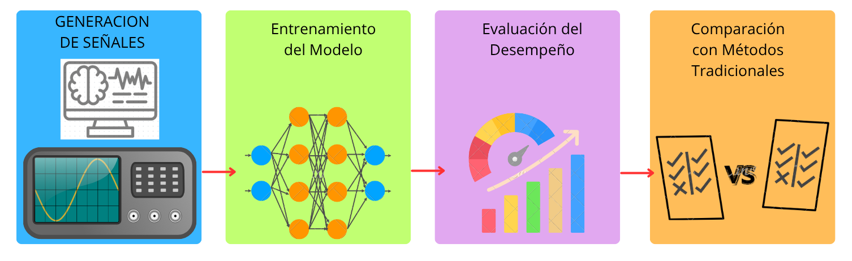
\includegraphics[scale=0.5]{figures/met/metodologia.png}
    \caption{Métodologia propuesta}
    \label{fig:met}
    \end{figure}

    Para abordar el problema inverso de localización de fuentes cerebrales a partir de señales EEG, se propone una metodología híbrida que integra modelos físicos de simulación, redes neuronales profundas y métricas de evaluación cuantitativa. Esta aproximación busca superar las limitaciones de los métodos clásicos mediante la incorporación de aprendizaje automático entrenado con datos simulados de alta fidelidad.

    \subsection{Generación de Datos Simulados}

    La primera etapa consiste en la creación de un conjunto de datos sintéticos que sirva como base de entrenamiento y validación del modelo. Para ello, se define un modelo de cabeza que representa las propiedades geométricas y de conductividad de los tejidos (cerebro, líquido cefalorraquídeo, cráneo y piel). Se consideran diferentes configuraciones, entre ellas:

    \begin{itemize}
    \item Modelo homogéneo: idealizado, de baja complejidad computacional.
    \item Método de elementos de frontera (BEM por sus siglas en inglés): solución numérica sobre mallas triangulares.
    \item Método de los Elementos Finitos (FEM por sus siglas en inglés): mayor precisión anatómica y flexibilidad geométrica.
    \item Modelo Localmente Esférico con Restricciones Anatómicas (LSMAC por sus siglas en inglés): aproximación esférica localmente adaptada a la anatomía.
    \end{itemize}

    El modelo de fuente define la distribución, orientación y dinámica temporal de los generadores neuronales. La actividad neuronal se modela mediante señales simples (como sinusoides) o patrones complejos generados con Neural Mass Models (NMMs), permitiendo simular potenciales evocados o actividad oscilatoria.

    Posteriormente, se resuelve el problema directo mediante el cálculo del lead field matrix, el cual permite proyectar la actividad de las fuentes a los sensores. A los datos generados se les añade ruido gaussiano controlado para simular condiciones reales.

    \subsection{Entrenamiento del Modelo de Deep Learning}

    Con los datos simulados se entrena una red neuronal profunda supervisada. La entrada del modelo consiste en señales EEG multicanal, y la salida corresponde a una estimación tridimensional de las fuentes activas. La arquitectura propuesta puede incluir:

    \begin{itemize}
        \item Redes convolucionales (CNN) para extracción de patrones espaciales.
        \item Redes recurrentes (RNN o LSTM) para capturar información temporal.
        \item Módulos de atención para mejorar la interpretación y localización.
    \end{itemize}

    El entrenamiento se realiza minimizando una función de pérdida compuesta por errores de localización y amplitud, con regularización para evitar sobreajuste.

    \subsection{Evaluación del Desempeño}

    Para validar la eficacia del modelo, se utilizarán métricas cuantitativas reconocidas en la literatura:

    \begin{itemize}
        \item \textbf{Localization Error (LE)}: distancia entre fuente estimada y real.
        \item \textbf{Temporal Error (TE)}: desviación entre los tiempos pico estimado y verdadero.
        \item \textbf{nMSE (Normalized Mean Squared Error)}: error cuadrático medio relativo.
        \item \textbf{PSNR (Peak Signal-to-Noise Ratio)}: calidad de la señal reconstruida.
        \item \textbf{Precision, Recall y F1-score}: para evaluar la detección correcta de regiones activas.
    \end{itemize}
    
    En el caso de datos reales, donde no se dispone de la “verdad conocida”, se utilizarán referencias clínicas como registros de iEEG o áreas de resección quirúrgica, así como comparación con modalidades complementarias como fMRI o PET.
    
    \subsection{Comparación con Métodos Tradicionales}
    
    Los resultados obtenidos serán comparados con los de técnicas clásicas de localización, como MNE, sLORETA y VARETA, utilizando el mismo conjunto de datos simulados y reales. Esta comparación permitirá establecer mejoras en términos de precisión espacial, temporal y robustez frente al ruido.


\subsection{Consideraciones Éticas}

Para el desarrollo de nuestro generador de señales así como la implementación de nuestro modelo se parte de bases de datos de EEG públicas de plataformas abiertas (como PhysioNet\cite{physionet2021auditoryeeg} o BNCI-Horizon 2020\cite{bnci2020datasets}). Las fuentes de estas bases de datos son abiertas y de uso libre para investigación por lo que no se requieren permisos o licencias especiales. Dado que esta información no recolecta información de fuentes primarias siendo datos de seres humanos no sera requerida consideraciones éticas extras. Las señales EEG utilizadas son datos públicos anonimizados y servirán exclusivamente como referencia para generar simulaciones sintéticas bajo condiciones controladas.
